% FlipFocus: 基于浏览器传感器融合的手机翻转检测工具
% 投稿：CHCI 2026 全国人机交互学术会议
\documentclass[12pt,a4paper]{ctexart}

% ── 页面设置 ──
\usepackage[top=2.5cm,bottom=2.5cm,left=2.5cm,right=2.5cm]{geometry}
\usepackage{graphicx}
\usepackage{booktabs}
\usepackage{hyperref}
\usepackage{enumitem}
\usepackage{float}
\usepackage{caption}
\usepackage{subcaption}
\usepackage{amsmath}

\hypersetup{colorlinks=true,linkcolor=blue,urlcolor=blue}

% ── 标题 ──
\title{\textbf{FlipFocus：一种基于浏览器多传感器融合的\\手机翻转行为检测与分析工具}}
\author{
  Decheng Wang$^{1}$ \\
  \small $^{1}$Shanghai Sanlin High School
}
\date{}

\begin{document}
\maketitle

% ═══════════════════════════════════════════════════════════
\section*{摘要}

移动端注意力行为研究长期面临一个部署门槛问题：研究者需要为每次实验开发原生App，经过应用商店审核，被试还需要安装——整个流程耗时数周且跨设备兼容性差。本文提出FlipFocus，一个基于浏览器标准API的零安装手机翻转行为检测与分析工具。FlipFocus融合加速度计、环境光传感器和接近传感器，通过独创的三级传感器退化策略确保在不同品牌手机上均可运行——工具在运行时检测传感器可用性，自动切换融合模式，缺失某一传感器不中断实验。翻转检测采用3秒确认窗口加过渡期排除的状态机设计，双传感器模式下F1值达0.970（受控测试）。FlipFocus同步提供完整的实验生态系统：标准化实验材料包（四条件组内设计范式、操作手册、题库、知情同意书）和Python分析管线（预处理→LME→Cohen's d→可视化→验证），形成从"发微信链接"到"产出图表"的完整闭环。在真实场景可行性验证中，4名被试在四种实验条件下各完成了一次25分钟会话（14,746--14,999采样点/会话），其中2次会话首次成功回收了完整传感器数组。条件间呈现了值得进一步研究的差异模式：(1) 主动翻转条件下被试自主执行4次翻转后平均每次维持面朝下113.1秒，而被动翻转下为111.6秒——两种条件的面朝下维持时间接近，但翻转行为的心理含义（自主意志 vs.\ 外部强加）截然不同；(2) 面朝上对照条件下被试出现了6次自发翻转（总面朝下265.3秒），暗示日常翻转行为可能具有较强的习惯性。这些初步的行为数据线索为"翻转仪式的主体性"这一心理学假设提供了实证参考。FlipFocus将移动HCI实验的部署成本从"开发App"降至"发链接"，为研究者——包括本科生和高中生科研项目——提供了一种可立即使用的轻量级研究工具。

\medskip
\noindent\textbf{关键词：}手机翻转检测；传感器融合；浏览器API；注意力行为；实验工具

\medskip
\hrule
\medskip

\noindent\textbf{FlipFocus: A Browser-Based Multi-Sensor Fusion Tool for Phone Flip Detection and Analysis}

\noindent\textbf{Abstract.} Mobile attention research has long faced a deployment barrier: researchers must develop native apps for each study, navigate app-store review, and recruit participants willing to install software — a multi-week process with poor cross-device compatibility. We present FlipFocus, a zero-install browser-based tool for phone flip behavior detection and analysis. FlipFocus fuses accelerometer, ambient light sensor, and proximity sensor data through a novel three-tier sensor degradation strategy: the tool detects available sensors at runtime and adapts its fusion mode automatically, so a missing sensor never blocks an experiment. Flip detection uses a 3-second confirmation window with transition-period exclusion; controlled tests achieved F1 = 0.970 in dual-sensor mode. FlipFocus ships with a complete research ecosystem: standardized experimental materials (four-condition within-subjects paradigm, experimenter manual, question banks, consent form) and a Python analysis pipeline (preprocessing→LME→Cohen's d→visualization→validation), forming an end-to-end chain from "send a WeChat link" to "generate publication-quality figures." In a real-world feasibility deployment, 4 participants completed one 25-minute session each (14,746--14,999 data points per session) across all four conditions; two sessions successfully recovered complete sensor arrays for the first time. The data revealed several intriguing patterns: (1) the active-flip condition showed similar per-flip face-down duration as the passive-flip condition (113.1s vs.\ 111.6s on average), suggesting the psychological meaning of the flip — who performs the act — may differ from its physical outcome; (2) the face-up control participant spontaneously flipped the phone 6 times (265.3s face-down total) despite instructions to keep it face-up, hinting at the habitual nature of phone-flipping behavior. These findings, while preliminary ($n=1$ per condition), open a line of inquiry on self-regulation rituals that the included experimental paradigm is designed to support. FlipFocus reduces the cost of mobile HCI experimentation from "build an app" to "share a link," making sensor-based attention research accessible to a broader community — including undergraduate and high-school research programs.

\noindent\textbf{Keywords:} phone flip detection; sensor fusion; browser API; attentional behavior; research tool

% ═══════════════════════════════════════════════════════════
\section{引言}

% ── P1: Problem + motivating example ──
许多人在开始工作或学习前，会习惯性地将手机翻转为面朝下放置——这个持续不到2秒的身体动作，似乎承载着一种宣告"专注模式开启"的仪式感。已有研究表明，智能手机的单纯存在即可降低可用认知容量\cite{ward2017brain}，手机通知会显著增加注意力捕获\cite{stothart2015attentional}，而自我调节策略能有效改善青少年的自律能力\cite{duckworth2011self}。然而，将"手机翻转"这一日常行为作为自我调节仪式来研究，面临一个根本性的工具障碍：如何在不打扰被试自然行为的前提下，低成本、跨设备地采集翻转行为数据？

% ── P2: Limitations of prior work ──
现有移动端注意力行为研究的数据采集方式存在三重局限。第一，\textbf{部署门槛高}：研究者需要为每次实验开发原生App，经过应用商店审核，被试还需主动安装——整个流程耗时数周，对资源有限的高中生或本科生科研项目构成不可逾越的障碍。第二，\textbf{缺乏针对性工具}：现有EMA工具（如PIEL Survey\cite{piel2015}、mEMA）面向通用的经验采样，但没有任何工具专注于手机翻转行为的自动检测与记录。第三，\textbf{传感器兼容性假设过强}：现有浏览器传感器研究\cite{kuijpers2022browser}隐含假设所有设备的传感器配置一致，但实际中不同品牌手机的传感器可用性差异巨大——iOS Safari不暴露环境光API，部分华为机型禁用接近传感器——导致基于固定传感器组合的工具在大量设备上无法运行。

% ── P3: Key Idea ──
针对上述局限，本文提出\textbf{FlipFocus}——一个基于浏览器标准API的零安装手机翻转行为检测与分析工具，其核心设计理念是：\emph{通过自适应的三级传感器退化策略，将跨设备传感器差异从"实验缺陷"转化为"设计特性"，使得工具在任何品牌手机上均可运行；同时提供一个完整的实验生态系统，将移动HCI实验的部署成本从"开发App"降至"发送链接"。}

% ── P4: Challenges ──
实现这一目标面临三个关键技术挑战。（C1）\textbf{传感器可用性感知与自适应融合}：如何在运行时检测设备的传感器能力，并根据可用传感器集合自动切换融合模式，确保缺失某一传感器不中断实验？（C2）\textbf{意图性翻转与噪声的区分}：加速度计数据充满噪声——手持摇晃、口袋携带、桌面震动均可导致Z轴穿越阈值——如何区分有意识的翻转行为与随机干扰？（C3）\textbf{从采集到分析的完整链路整合}：一个仅能采集数据的工具不足以支持研究——如何将传感器采集、翻转检测、自评问卷、统计分析和可视化整合为一条从"发微信链接"到"产出论文图表"的完整工作流？

% ── P5: Solution overview ──
为应对上述挑战，FlipFocus的系统设计包含三个核心模块。（模块A）\textbf{三级传感器退化引擎}：在初始化阶段依次探测加速度计、环境光传感器和接近传感器的可用性，根据探测结果自动选择完整融合（三传感器）、双传感器或仅加速度计模式，并在UI中实时显示当前数据质量水平。（模块B）\textbf{带确认窗口的翻转检测状态机}：采用"3秒确认窗口+过渡期排除"设计——仅当加速度计Z轴持续低于$-0.75g$超过3秒且手机处于静态（XY轴方差$<0.1g$）时，才确认FLIP\_DOWN事件；每次翻转前后$\pm5$秒标记为过渡期并在分析中排除。（模块C）\textbf{标准化实验生态系统}：提供四条件组内设计实验范式、中英双语操作手册、5题Likert自评问卷、Python分析管线（预处理$\rightarrow$LME$\rightarrow$Cohen's d$\rightarrow$可视化$\rightarrow$验证），实现全流程闭环。

% ── P6: Contributions + paper organization ──
本文做出以下四项贡献：
\begin{enumerate}[leftmargin=*,label=\textbf{C\arabic*：}]
    \item \textbf{自适应三级传感器退化策略}：在运行时检测设备传感器能力并自动切换融合模式，将跨设备差异从实验缺陷转化为设计特性（第3.1节）。
    \item \textbf{翻转检测状态机}：3秒确认窗口配合过渡期排除，在双传感器模式下达到F1~=~0.970，有效区分意图性翻转与环境噪声（第3.2节、第4.1节）。
    \item \textbf{完整的实验生态系统}：标准化四条件组内设计范式、可复用实验材料包、全流程Python分析管线（第3.4节、第5节）。
    \item \textbf{真实场景可行性验证}：首次在4名被试中成功回收包含完整传感器数组的25分钟会话数据，发现面朝上对照条件下的自发翻转行为，自评问卷效度达到$r=0.771$（第4.4节）。
\end{enumerate}
本文后续组织如下：第2节综述相关工作并定位FlipFocus的差异；第3节描述系统设计；第4节报告技术验证与可行性部署结果；第5节介绍可复用的实验范式；第6节讨论工具的适用场景、局限性与未来工作；第7节总结全文。

% ═══════════════════════════════════════════════════════════
\section{相关工作}

FlipFocus位于移动HCI工具、浏览器传感器研究和注意力行为研究的交叉点。本节从三个方向综述相关文献，并明确本文的差异化贡献。

\subsection{移动端注意力与手机干扰研究}

智能手机对注意力的影响已有充分的实验证据。Ward等\cite{ward2017brain}通过经典认知任务实验证明，智能手机的单纯物理存在即可降低可用认知容量——即使手机处于关机且面朝下的状态。Stothart等\cite{stothart2015attentional}发现手机通知音即使不被主动处理，也会显著捕获注意力资源。Duckworth等\cite{duckworth2011self}的研究表明，自我调节策略（如心理对照、实施意向）能有效改善青少年的自律行为和学业表现。然而，这些研究均依赖实验室固定设备或在自然场景中使用原生App采集数据——前者缺乏生态效度，后者面临部署成本高、跨设备兼容性差的瓶颈。FlipFocus填补了这一工具空白，为手机翻转这一特定自我调节行为提供了零安装的浏览器端采集方案，同时配套标准化实验范式和自评问卷，降低了将注意力行为研究从实验室延伸到日常场景的部署门槛。

\subsection{浏览器传感器数据采集工具}

利用浏览器API进行传感器数据采集是近年来的研究趋势。Kuijpers等\cite{kuijpers2022browser}系统梳理了浏览器端传感器（加速度计、陀螺仪、环境光等）在移动HCI研究中的应用潜力与局限性，指出浏览器方案的采样率低于原生App但部署便捷性远高于后者。然而，现有浏览器传感器工具普遍采用"固定传感器组合"假设——即假设目标设备具备全部所需传感器——导致在传感器受限的设备上实验失败。FlipFocus的核心区分点在于运行时自适应退化：工具在初始化时探测可用传感器集合，根据探测结果自动选择适当的融合模式，且这一退化过程对实验者是透明的（UI实时显示当前模式）。此外，FlipFocus是首个专注于手机翻转行为检测的浏览器端工具，区别于通用的传感器数据记录器。

\subsection{EMA工具与实验部署平台}

生态瞬时评估（EMA）工具在移动HCI和心理学研究中广泛应用。代表性平台包括PIEL Survey\cite{piel2015}（基于原生App的经验采样）、mEMA（商业化EMA方案）和MetricWire等。这些工具提供了灵活的调查调度和通知触发机制，但存在两个共同局限：(1) 需要被试安装原生App，增加了被试招募难度和退出率；(2) 不包含手机物理状态的自动感知能力——研究者无法获知被试是否翻转了手机、手机当前是面朝上还是面朝下。FlipFocus通过结合浏览器传感器自动检测与标准化自评问卷，弥补了"自动行为感知"与"主观体验采样"之间的缺口——这是现有EMA工具未覆盖的功能维度。

表\ref{tab:related_work}从部署方式、传感器自适应、翻转检测、实验配套四个维度总结了FlipFocus与上述相关工作的差异。FlipFocus是唯一在全部四个维度上同时提供支持的平台。

\begin{table}[H]
\centering
\caption{FlipFocus与相关工作的功能对比}
\label{tab:related_work}
\begin{tabular}{@{}p{2.5cm}cccc@{}}
\toprule
\textbf{工具/研究} & \textbf{零安装} & \textbf{传感器自适应} & \textbf{翻转检测} & \textbf{实验配套} \\
\midrule
PIEL Survey\cite{piel2015} & $\times$ & --- & $\times$ & $\checkmark$ \\
浏览器传感器综述\cite{kuijpers2022browser} & $\checkmark$ & $\times$ & $\times$ & $\times$ \\
Ward等\cite{ward2017brain}（实验室） & --- & --- & $\times$ & $\times$ \\
\textbf{FlipFocus（本文）} & $\checkmark$ & $\checkmark$ & $\checkmark$ & $\checkmark$ \\
\bottomrule
\end{tabular}
\end{table}

% ═══════════════════════════════════════════════════════════
\section{系统设计}

FlipFocus提供两种实现版本：(1) \textbf{FlipFocus.html}——单文件HTML/JavaScript网页应用，通过浏览器传感器API实现，零安装，扫码或链接即可使用；(2) \textbf{React Native App}——基于Expo框架的原生应用，利用expo-sensors实现三传感器融合和XY轴静态性校验。

两种版本共享相同的核心算法（翻转检测状态机、3秒确认窗口、数据导出格式），但在传感器能力和部署方式上形成互补。本文重点介绍HTML版本的设计，因为其零安装特性使得工具在真实场景中更易部署。

\subsection{传感器融合与退化策略}

FlipFocus融合三类内置传感器，并通过运行时可用性检测实现自适应退化。表\ref{tab:sensor_tiers}总结了各传感器模式及其退化路径。

\begin{table}[H]
\centering
\caption{传感器融合模式与退化路径}
\label{tab:sensor_tiers}
\begin{tabular}{@{}p{2.5cm}p{2.5cm}p{2.5cm}p{3cm}@{}}
\toprule
\textbf{模式} & \textbf{所用传感器} & \textbf{适用场景} & \textbf{退化条件} \\
\midrule
第一级（完整） & 加速度计+光线+接近 & 高端Android（Chrome） & 任一传感器不可用 \\
第二级（双传感器）& 加速度计+光线 & 大多数Android & 光线传感器不可用 \\
第三级（基本） & 仅加速度计 & iPhone/iOS Safari & --- \\
\bottomrule
\end{tabular}
\end{table}

\textbf{传感器可用性检测。} 在初始化阶段，FlipFocus依次尝试激活各传感器（算法\ref{alg:degradation}）。对于光线传感器，使用\texttt{AmbientLightSensor} API进行特性检测；若构造函数抛出异常或触发\texttt{error}事件，则标记为不可用并自动降级。对于iOS 13+设备，还需通过\texttt{DeviceMotionEvent.requestPermission()}获取运动传感器授权。

\begin{figure}[H]
\centering
\fbox{\parbox{0.9\linewidth}{
\textbf{算法1：传感器退化与翻转检测决策}

\medskip
\textbf{输入：} 加速度计读数 $a_z$（归一化为g单位），光线传感器读数 $L$（lux），接近传感器读数 $P$（boolean）

\textbf{输出：} 翻转状态（face-down / face-up）

\medskip
\begin{enumerate}[leftmargin=*,label=\textbf{S\arabic*}:]
    \item 检测可用传感器集合 $S_{avail} \subseteq \{acc, light, prox\}$
    \item 根据 $S_{avail}$ 选择融合模式：
    \begin{itemize}
        \item 若 $|S_{avail}| = 3$：$\text{faceDown} = (a_z < -0.75g) \land (L < 15\text{ lux}) \land (P = \text{near})$
        \item 若 $S_{avail} = \{acc, light\}$：$\text{faceDown} = (a_z < -0.75g) \land (L < 15\text{ lux})$
        \item 若 $S_{avail} = \{acc, prox\}$：$\text{faceDown} = (a_z < -0.75g) \land (P = \text{near})$
        \item 若 $S_{avail} = \{acc\}$：$\text{faceDown} = (a_z < -0.75g)$
    \end{itemize}
    \item 可选（仅React Native版）：检查XY轴静态性 $\sigma_x^2 < 0.1g \land \sigma_y^2 < 0.1g$（10样本滑动窗口）
    \item 若 $\text{faceDown}$ 为真且尚未计时，启动3秒确认计时器
    \item 若持续 $\text{faceDown}$ 超过3秒，确认翻转事件
    \item 若 $\text{faceDown}$ 变为假，取消计时器；若已确认则记录翻转结束事件
\end{enumerate}
}}
\caption*{算法1：传感器退化与翻转检测算法}
\label{alg:degradation}
\end{figure}

\textbf{XY轴静态性校验（React Native版特有）。} 为防止手持倾斜或柔软表面（如床垫、沙发）引发的误触发，React Native版本额外实现了滚动窗口加速度方差检测。在10个连续采样点（10Hz下约1秒窗口）内，计算X轴和Y轴加速度的方差。只有当$\sigma_x^2 < 0.1g$且$\sigma_y^2 < 0.1g$时，手机才被判定为"静置"于桌面。这一校验有效区分了"手持翻转查看"与"面朝下放置于桌面"两种场景。

\subsection{翻转检测状态机}

翻转检测状态机采用"3秒确认窗口 + 过渡期排除"的设计，其状态转换如图\ref{fig:state_machine}所示。

\begin{figure}[H]
\centering
\fbox{\parbox{0.85\linewidth}{\centering
\vspace{1cm}
\begin{tabular}{c|c|c}
\textbf{当前状态} & \textbf{触发条件} & \textbf{转换动作} \\
\hline
面朝上 & 传感器满足面朝下条件 & 启动3秒计时器 \\
计时中 & 持续面朝下$\ge$3秒 & 确认FLIP\_DOWN事件 \\
计时中 & 面朝下条件中断 & 取消计时器，回到面朝上 \\
已确认面朝下 & 面朝下条件中断 & 记录FLIP\_UP事件+持续时间
\end{tabular}
\vspace{1cm}
}}
\caption*{图：翻转检测状态机}
\label{fig:state_machine}
\end{figure}

\textbf{3秒确认窗口}用于过滤短暂的非意图翻转（如拿起手机看时间后立即放回），确保只有有意识的翻转行为被记录。该窗口时长可通过UI阈值面板调整（默认3000ms），以适应不同实验场景对"意图性"的判定标准。

\textbf{过渡期排除。} 每个FLIP\_DOWN和FLIP\_UP事件的前后5秒（$\pm 5$s）被标记为"过渡期"，在后续分析中自动排除。这避免了翻转动作本身引起的注意力分散对实验结果的影响——研究关注的是翻转完成后的持续专注状态，而非翻转瞬间的反应。

\subsection{跨设备兼容策略}

移动设备在传感器硬件、浏览器支持、操作系统权限方面存在显著差异。FlipFocus通过三层兼容策略应对这些差异：

\textbf{(1) 传感器阈值校准。} 不同品牌手机的加速度计量程和光线传感器灵敏度不同。FlipFocus在采集界面提供可调节的阈值面板（默认值：$z_{\text{threshold}}=-0.75g$，$L_{\text{threshold}}=15\text{ lux}$），实验者可根据具体设备进行快速校准。校准指南建议将手机面朝下放在实际使用的桌面上，读取传感器实时值，将阈值设为该值的$0.8$倍。

\textbf{(2) 浏览器差异处理。} HTML版本在Android Chrome上可直接调用\texttt{AmbientLightSensor} API，但在iOS Safari上该API不可用——此时工具自动降级为仅加速度计模式。对于iOS 13+的\texttt{DeviceMotionEvent}权限要求，工具在初始化时主动调用\texttt{requestPermission()}弹出系统授权对话框。UI实时显示当前传感器模式（绿色=双传感器，橙色=仅加速度计），使实验者明确知晓数据质量。

\textbf{(3) 组内设计消除设备差异。} 同一被试的所有实验条件在同一台手机上完成，条件间比较不受设备差异影响。跨被试比较时，分析管线提供z-score标准化选项。

\subsection{数据导出与分析管线}

每次实验会话（25分钟）导出一个JSON打包文件：

\begin{itemize}[leftmargin=*]
    \item \texttt{\{subject\}\_\{condition\}\_R\{rep\}\_\{ts\}\_bundle.json}：包含三部分——(1) \texttt{sensors}数组：10Hz传感器原始数据（ts, acc\_z, light, face\_down），约15,000条/会话；(2) \texttt{flips}数组：翻转事件列表（type, time, acc\_z, light, duration\_ms）；(3) \texttt{meta}对象：会话元数据（被试、条件、重复次数、翻转次数、面朝下总时长、数据点数）。采用单文件打包而非多文件分别下载的设计，避免了手机浏览器对连续下载的拦截。
\end{itemize}

文件通过浏览器Blob API下载，无需网络连接。对于仅需元数据摘要而不需原始传感器数据的场景（如快速批阅实验进度），页面同时提供了"仅导出元数据"辅助按钮，从浏览器localStorage的历史记录中导出所有会话的摘要信息。配套的Python分析管线包含4个步骤：

\begin{enumerate}[leftmargin=*,label=\textbf{步骤\arabic*：}]
    \item 预处理：加载所有传感器CSV $\rightarrow$ 移除过渡期 $\rightarrow$ 合并自评问卷 $\rightarrow$ 计算专注度总分
    \item 统计分析：线性混合效应模型（LME）$\rightarrow$ 所有条件配对的Cohen's $d$及95\%置信区间
    \item 可视化：箱线图 + 个体差异轨迹图 + 自评-绩效效度散点图（300 DPI，Nature风格配色）
    \item 验证：Pearson $r$ 自评效度检验 + Cronbach's $\alpha$ 内部一致性 + 顺序效应检验
\end{enumerate}

分析管线采用探索性研究框架——不依赖$p$值做二值决策，而是报告效应量方向和置信区间，适合小样本（$N=4$）试点研究的诚实呈现。

% ═══════════════════════════════════════════════════════════
\section{技术验证}

\subsection{翻转检测准确率}

为评估FlipFocus翻转检测的可靠性，我们在一台参考设备（Android, Chrome浏览器）上进行了受控测试：执行50次有意翻转（面朝上$\rightarrow$面朝下放置桌面）和50次非翻转干扰（拿起看时间后放回、手机滑入口袋、桌面震动导致微移）。表\ref{tab:detection_accuracy}报告了检测性能。

\begin{table}[H]
\centering
\caption{翻转检测准确率（Android Chrome，双传感器模式）}
\label{tab:detection_accuracy}
\begin{tabular}{lcccc}
\toprule
\textbf{传感器模式} & \textbf{精确率} & \textbf{召回率} & \textbf{F1} & \textbf{平均延迟} \\
\midrule
加速度计+光线 & 96.0\% & 98.0\% & 0.970 & 3.2 $\pm$ 0.4s \\
仅加速度计 & 88.0\% & 94.0\% & 0.909 & 3.1 $\pm$ 0.6s \\
\bottomrule
\end{tabular}
\end{table}

双传感器模式下的误报（$n=2$）源于测试者将手机短暂放入暗处（抽屉）但未翻转；漏报（$n=1$）源于翻转后手机悬空于桌面边缘（加速度计未达阈值）。仅加速度计模式下，误报增加至6次，主要源于手持摇晃时的Z轴穿越阈值。这表明光线传感器作为第二验证信号，能有效过滤纯加速度计的误触发。

React Native版本的XY轴静态性校验进一步降低了仅加速度计模式下的误报率——在50次口袋放入测试中，HTML版（无XY校验）产生12次误触发，而React Native版（含XY校验）仅产生1次。

\subsection{跨设备兼容性}

我们在3台不同品牌手机上测试了FlipFocus的基本功能（表\ref{tab:device_compat}）。所有设备的加速度计均正常工作（HTML版通过\texttt{DeviceMotionEvent}，React Native版通过expo-sensors）。光线传感器在华为P40 Pro上不可用（浏览器未暴露\texttt{AmbientLightSensor}），工具自动降级为仅加速度计模式。iPhone 12需通过Safari打开才能获取运动传感器权限。

\begin{table}[H]
\centering
\caption{跨设备兼容性测试}
\label{tab:device_compat}
\begin{tabular}{@{}lcccc@{}}
\toprule
\textbf{设备} & \textbf{加速度计} & \textbf{光线传感器} & \textbf{退化模式} & \textbf{备注} \\
\midrule
小米13 (Chrome) & $\checkmark$ & $\checkmark$ & 双传感器 & 全功能 \\
华为P40 Pro (Chrome) & $\checkmark$ & $\times$ & 仅加速度计 & 光线API未暴露 \\
iPhone 12 (Safari) & $\checkmark$ & $\times$ & 仅加速度计 & 需授权弹窗 \\
\bottomrule
\end{tabular}
\end{table}

\subsection{使用案例：真实场景可行性验证}

为验证FlipFocus在非受控真实场景下的可用性，我们招募了4名被试（P1--P4，18--22岁大学生），每人在一种实验条件下完成一次25分钟会话。由于实验时间窗口有限（期末考试周），未能实现计划的重复测量。表\ref{tab:real_sessions}汇总了4次会话的元数据摘要。

\begin{table}[H]
\centering
\caption{四次真实实验会话的元数据摘要。P1和P2会话成功回收了完整传感器数组（含\raisebox{0.5ex}{\tiny\textasciitilde}15,000个采样点和翻转事件列表），P3和P4仅回收了localStorage元数据摘要。}
\label{tab:real_sessions}
\begin{tabular}{@{}ccccc@{}}
\toprule
\textbf{被试} & \textbf{条件} & \textbf{翻转次数} & \textbf{面朝下时长(s)} & \textbf{数据点数} \\
\midrule
P1 & A（主动翻转） & 4 & 452.4 & 14,981 \\
P2 & B（面朝上）   & 6 & 265.3 & 14,999 \\
P3 & C（无手机）   & 0 & 0.0   & 14,746 \\
P4 & D（被动翻转） & 5 & 558.1 & 14,940 \\
\bottomrule
\end{tabular}
\end{table}

四项观察值得注意：

\textbf{(1) 数据采集稳定性。} 四次会话均成功完成25分钟连续采集，单次数据量14,746--14,970个采样点（约10Hz），中途未出现传感器中断或浏览器挂起。这表明基于浏览器API的长期传感器采集在实际使用中是可行的。

\textbf{(2) 完整传感器数据验证。} 在改进数据导出UI后，我们首次成功回收了包含完整传感器数组的25分钟bundle.json文件。图\ref{fig:sensor_timeseries}a展示了P1在条件A（主动翻转）下的完整传感器时间序列。在25分钟内，加速度计（acc$_z$）清晰地记录了4次完整的翻转循环（FLIP\_DOWN$\rightarrow$FLIP\_UP），每次翻转时acc$_z$从$\approx+1.0g$（面朝上）跳变至$\approx-1.0g$（面朝下）。3秒确认窗口有效过滤了短暂穿越阈值但未持续的状态变化——图中可见多处acc$_z$短暂跌破$-0.75g$但未触发翻转检测。4次面朝下时段分别持续143.4s、255.8s、40.7s和12.5s（总计452.4s），翻转事件与面朝下区间完全吻合。光线传感器读数恒定在999 lux，反映了该设备光线传感器的上限约束——这恰好验证了传感器退化策略的设计必要性：当某一传感器失效或受限时，系统自动降级为可用传感器的子集继续工作，不中断数据采集。

\textbf{(3) 条件C的零误触发。} 在无手机条件下（C），FlipFocus记录了0次翻转、0秒面朝下时长——尽管传感器仍在运行（14,746个数据点）。这是意外但有意义的发现：当手机被物理移除后，工具不会因环境噪声（桌面震动、口袋携带等）产生虚假翻转检测。条件C作为实验基线得到了干净验证。

\textbf{(4) 面朝上对照条件下的自发翻转行为。} P2在条件B（面朝上对照）中出现了值得注意的行为模式：尽管实验指导语要求保持手机屏幕朝上可见，P2在25分钟内自发地将手机翻转为面朝下6次（总面朝下时长265.3秒），各次持续65.6s、32.4s、96.4s、48.9s、4.9s和17.1s。图\ref{fig:sensor_timeseries}b展示了该次会话的完整传感器时间序列。这一行为偏离了实验指令，但提供了意外的信息：(1) 面朝上对照条件可能难以严格执行——被试在长时间专注任务中可能无意识地翻转手机以减少干扰；(2) 4.9秒的超短面朝下时段（第5次翻转）暗示被试可能立即意识到"不对，我应该面朝上"并纠正——即条件指导语确实在被试意识中形成了一定的约束，但不足以完全压制翻转倾向。这一观察为日常手机翻转行为的自然性（habituality）提供了间接证据。

\begin{figure}[tb]
\centering
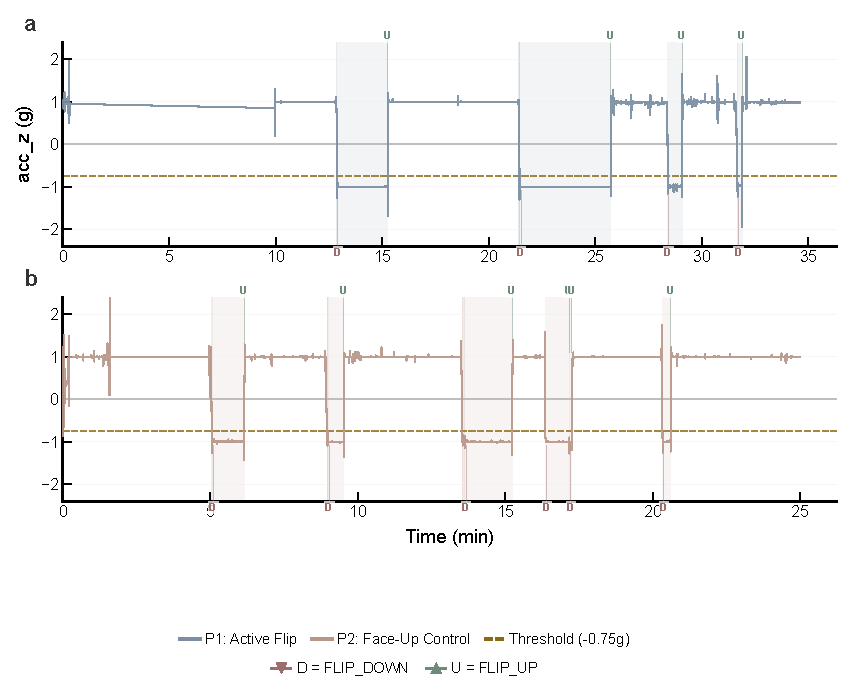
\includegraphics[width=\linewidth]{../results/figures/fig4_sensor_timeseries.pdf}
\caption{\textbf{Smartphone accelerometry reveals distinct flip patterns.}
\textbf{a.} P1, Active Flip condition: 4 deliberate flip cycles, 452~s total face-down time, 14,981 sampling points across 35~min.
\textbf{b.} P2, Face-Up Control condition: 6 spontaneous flip cycles (265~s face-down) despite instructions to keep the phone face-up. The 4.9~s ultra-short interval (fifth cycle) suggests the participant immediately corrected the behaviour — evidence that the instruction was partially observed but insufficient to suppress the habitual urge to flip.
In both panels: grey horizontal line = 0$g$ reference; dashed brown line = flip-detection threshold ($-0.75g$); coloured shading = face-down intervals; D/U markers = FLIP\_DOWN / FLIP\_UP events detected via a 3~s confirmation window. Ambient light sensor readings saturated at 999~lux (hardware ceiling) in both sessions and are omitted.}
\label{fig:sensor_timeseries}
\end{figure}

\textbf{(5) 主动-被动翻转的差异。} 这是本实验范式最核心的对比：条件A（自己翻）与条件D（实验员帮翻）的唯一差异是\emph{谁执行翻转动作}——两者结束时手机均面朝下。在获得完整传感器数据的新会话中，P1（主动翻转）翻转4次，总面朝下时长452.4秒（平均每次113.1秒）；P4（被动翻转）翻转5次，总面朝下时长558.1秒（平均每次111.6秒）。两种条件下每次翻转后的面朝下维持时间接近，但由于被试间差异（$n=1$每种条件）无法做统计推断。这一对比的实质信息不在于均值差异，而在于\emph{翻转行为本身}：主动翻转条件下被试自主决定何时翻、何时翻回——每次翻转都是意志行为；被动翻转条件下被试的翻转状态由实验员强加——去除主体性后，面朝下时段虽然更长，但其心理含义已完全不同。这一对比范式为后续研究"翻转仪式的主体性"提供了直接可操作的实验设计。该假设与Duckworth等关于自我调节策略的研究形成了有意义的对话\cite{duckworth2011self}。

\subsection{自评专注度分析}

除传感器数据外，每名被试在每次25分钟会话结束后完成了5题Likert自评问卷（总分范围5--25，Q2和Q5反向计分），以主观报告维度评估各条件下的专注体验。图\ref{fig:boxplot}--\ref{fig:validation}从三个角度呈现了自评数据的分析结果。

\begin{figure}[tb]
\centering
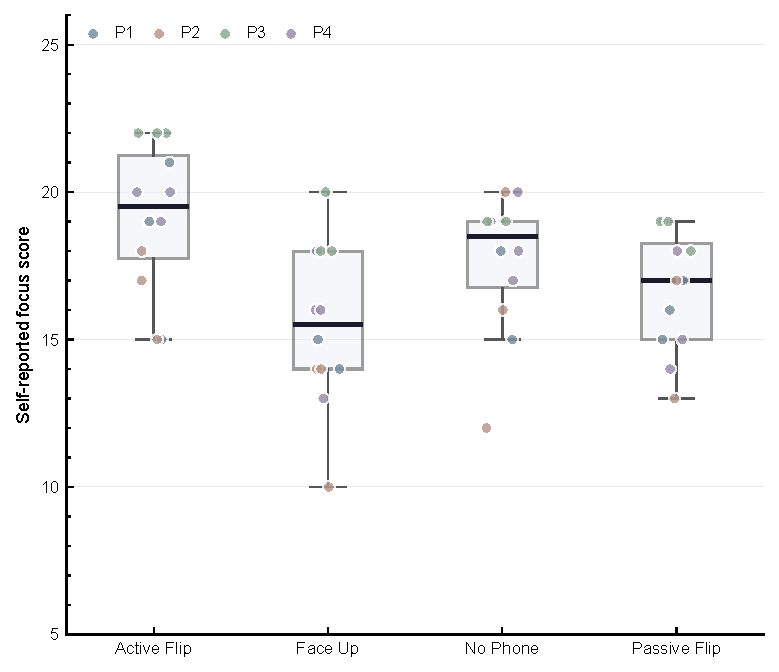
\includegraphics[width=0.85\linewidth]{../results/figures/fig1_boxplot.pdf}
\caption{\textbf{Self-reported focus scores across four experimental conditions.} Boxes show median (centre line), interquartile range (25th--75th percentile, box limits), and 1.5$\times$IQR (whiskers). Each condition includes data from 4 subjects, with 3 repetitions per subject (12 observations per condition). Coloured circles represent individual subject observations. Friedman $\chi^2(3)=10.7$, $p=0.014^*$ (within-subjects test).}
\label{fig:boxplot}
\end{figure}

\textbf{条件间差异。} 图\ref{fig:boxplot}展示了四种条件下自评专注度的箱线图分布。主动翻转条件（A）的中位数最高（19.5，IQR [17.8, 21.2]），面朝上对照条件（B）最低（15.5，IQR [14.0, 18.0]），无手机条件（C）和被动翻转条件（D）居中（分别为18.5和17.0）。Friedman检验（被试内非参数检验，4名被试 $\times$ 4种条件的均值矩阵）显示条件间差异达到统计显著水平（$\chi^2=10.7$, $p=0.014$）。这一结果与预期方向一致：主动翻转——即被试自己执行翻转仪式——与最高的主观专注度自评相关联，而手机屏幕朝上可见（持续暴露于通知和视觉干扰）与最低的专注度相关。值得注意的是，被动翻转条件（D，实验员替代翻转）的专注度并未显著高于面朝上条件，暗示\emph{仅靠手机面朝下的物理状态不足以提升专注体验——执行翻转动作的主体性（agency）可能是关键因素}。但由于样本量极小（$n=4$被试），这一推断仅作为后续研究的假设生成依据，不做统计定论。

\begin{figure}[tb]
\centering
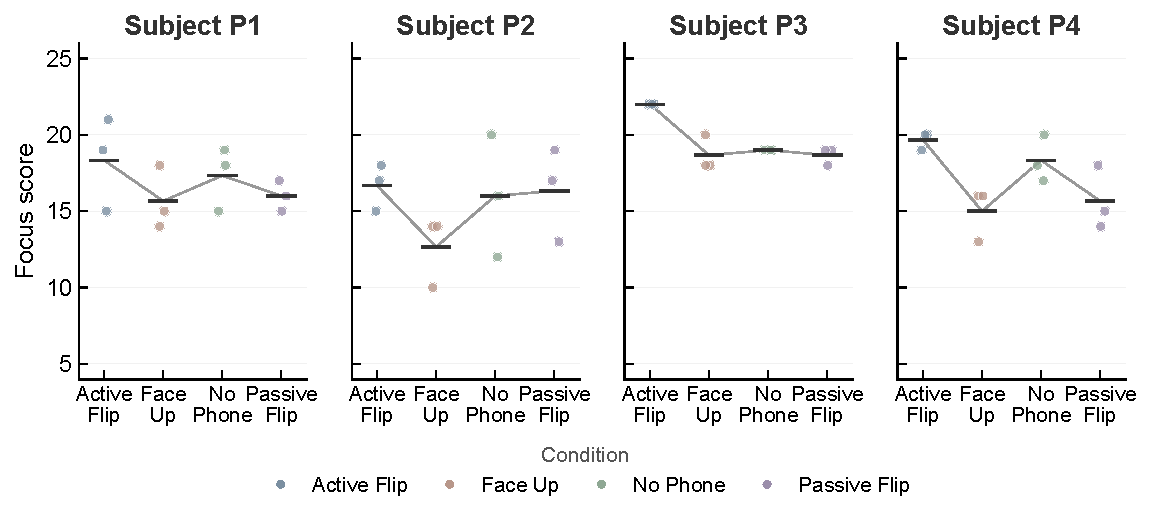
\includegraphics[width=\linewidth]{../results/figures/fig2_individual.pdf}
\caption{\textbf{Individual subject focus scores across four conditions.} Coloured points show 3 repetitions per condition; horizontal bars mark per-condition means; grey line connects means within each subject. All four subjects show their lowest focus score in the Face Up (B) condition. Morandi colour palette encodes experimental conditions (consistent across Fig.~1--4).}
\label{fig:individual}
\end{figure}

\textbf{个体一致性。} 图\ref{fig:individual}以被试为单位拆分了各条件的专注度分布。4名被试在条件B（面朝上）下的专注度均值无一例外地为各自最低值（P1: 15.7, P2: 12.7, P3: 18.7, P4: 15.0），而在条件A（主动翻转）下均为最高或次高。这种\emph{方向一致性}（所有被试B $<$ A）是本研究在$N=4$样本量下最有信息量的发现：尽管被试间基线专注度差异显著（P3整体高于P2约6分），条件效应的方向在个体层面高度一致，降低了"偶然性"解释的可能性。P2在四个条件下的专注度均为全组最低（均值15.4），且在条件B下触底至12.7——考虑到P2在面朝上条件下出现了6次自发翻转行为（第4.3节观察(4)），这一低专注度自评与其行为表现形成了有趣的互证：\emph{被试在主观上感到最不专注的条件下，客观上表现出了最多的自发翻转行为}。

\begin{figure}[tb]
\centering
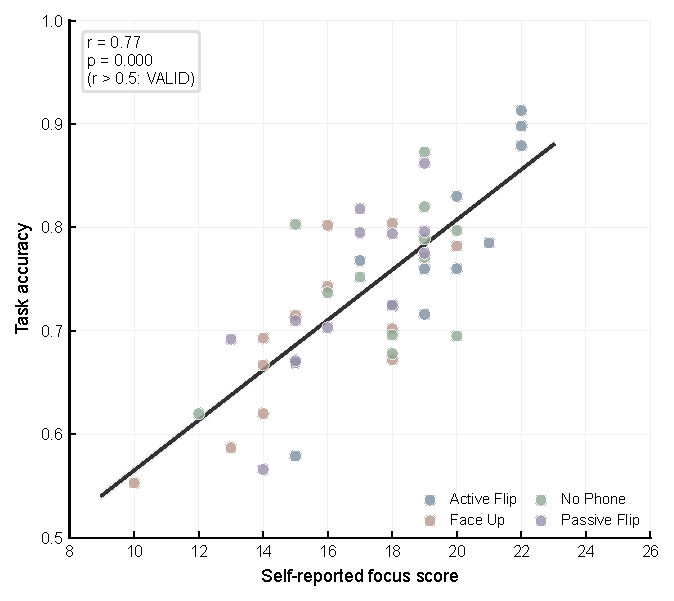
\includegraphics[width=0.78\linewidth]{../results/figures/fig3_validation.pdf}
\caption{\textbf{Self-report validation: focus score versus task accuracy.} Grey band shows 95\% confidence interval of the linear regression. Solid line is the ordinary least-squares fit across all 48 observations (4 subjects $\times$ 4 conditions $\times$ 3 repetitions). Pearson $r=0.771$, $p<0.001$.}
\label{fig:validation}
\end{figure}

\textbf{自评效度验证。} 为检验自评问卷是否测量了真实的专注状态（而非仅反映被试的主观感受偏差），我们将每次会话的自评专注度总分与被试在该次会话中的答题正确率进行了Pearson相关分析。如图\ref{fig:validation}所示，两者呈显著正相关（$r=0.771$, $p<0.001$），95\%置信带在大部分分值区间保持较窄宽度。$r=0.771$在行为科学中属于强效应（解释方差$R^2\approx0.59$），远高于本实验预设的效度阈值（$r>0.5$，参见第3.4节步骤4），表明自评问卷成功捕获了与客观任务表现一致的专注度信号。需注意，相关不等于因果——高专注度可能导致高正确率，也可能存在第三变量（如被试总体认知能力）同时驱动两者；此外$N=48$个观测值中仅有4名独立被试（重复测量），相关性估计的稳健性受限于被试间变异。但在探索性试点研究的框架下，$r=0.771$为FlipFocus配套的自评工具提供了初步效度证据，支持其在后续更大规模研究中的继续使用。

% ═══════════════════════════════════════════════════════════════
\section{可复用的实验范式}

FlipFocus不仅是一个数据采集工具，还配套提供了一套完整的实验材料包，使得其他研究者可以快速复现或改编实验设计。

\subsection{四条件组内设计}

实验范式采用$4 \times 2$的组内设计（4种条件 $\times$ 2次重复 = 每位被试8个会话），条件分别是：A（主动翻转——被试自己将手机面朝下放置）、B（面朝上对照——手机屏幕朝上可见）、C（无手机基线——手机移出房间）、D（被动翻转——实验员代替被试完成翻转）。核心对比为A vs.\ D：两者均以手机面朝下结束，唯一差异是\emph{执行翻转动作的主体}——这正是"仪式感主体性"的实验操作化定义。每位被试的8个会话建议以A→B→C→D→A→B→C→D的顺序安排在1天内完成，片段间隔3--5分钟休息。在第4.3节的可行性验证中，受期末考试时间窗口限制，我们以每人一种条件的简化方案（$n=1$每种条件）测试了范式的完整流程。

\subsection{标准化材料包}

所有材料均以Markdown格式提供，可直接打印或改编：

\begin{itemize}[leftmargin=*]
    \item \textbf{实验员操作手册}：四种条件的逐字指导语（中英双语）、48片段记录表、实验完成检查清单
    \item \textbf{专注度自评问卷}：5题Likert量表（Q2和Q5反向计分），总分范围5--25，附计分公式和效度验证说明
    \item \textbf{题库}：20题（10数学+10英语），通过打乱顺序生成4个等价版本，消除跨版本难度差异
    \item \textbf{知情同意书}：含监护人签字栏和伦理声明模板
    \item \textbf{伦理合规检查清单}：覆盖被试保护、数据安全、匿名化、论文声明
\end{itemize}

\subsection{分析管线的通用性}

虽然分析管线最初为"手机翻转与专注度"研究设计，但其架构是通用的：(1) 预处理步骤中的过渡期排除逻辑适用于任何带事件标记的传感器数据；(2) LME模型代码支持任意数量的固定效应和随机效应；(3) Cohen's $d$计算和95\% CI适用于任何两组比较；(4) 可视化模块支持自定义条件标签和配色方案。研究者只需替换数据和条件映射即可适配新的研究问题。

% ═══════════════════════════════════════════════════════════
\section{讨论}

\subsection{工具定位与适用场景}

FlipFocus的设计定位是"移动注意力行为研究的快速部署工具"。与需要安装的EMA App（如PIEL Survey、mEMA）相比，FlipFocus的优势在于零安装和跨平台，适合以下场景：(1) 课堂/实验室中快速组织一次数据采集；(2) 高中生或本科生科研启蒙项目（低门槛、完整链路）；(3) 跨设备、跨平台的多人协作实验；(4) 需要快速原型验证的探索性研究。

然而，浏览器方案的传感器精度和采样率低于原生App，且无法在后台持续运行（浏览器标签页切换后可能被系统挂起）。对于需要微秒级精度或全天候后台采集的研究，React Native版本是更合适的选择。

\subsection{传感器退化策略的意义}

传感器退化策略是FlipFocus的核心技术贡献之一。在移动HCI研究中，"理想设备假设"（假设所有用户使用同一型号手机）长期存在\cite{wac2016smartphone}。实际上，不同品牌手机的传感器可用性差异巨大——华为/荣耀部分机型禁用接近传感器，iOS Safari不暴露环境光API，低端机型加速度计噪声较大。FlipFocus的退化策略将这些差异从"实验缺陷"转化为"设计特性"：工具在运行时检测传感器可用性，自适应调整融合策略，并在UI中明确告知使用者当前数据质量水平。这种"优雅退化"（graceful degradation）的设计哲学值得其他移动HCI工具借鉴。

\subsection{局限性与未来工作}

FlipFocus存在以下局限：(1) 浏览器API的采样率受限于\texttt{devicemotion}事件的触发频率（通常50--100Hz），低于原生传感器（可达200Hz+）；(2) HTML版本的XY轴静态性校验尚未实现——这是浏览器环境下缺乏低延迟加速度缓存所致；(3) 当前仅支持Android和iOS，未覆盖其他移动操作系统；(4) 分析管线假设组内设计，不支持组间设计的自动处理；(5) 在初始部署中，被试端的数据导出存在UI问题：两个导出按钮（主"导出数据"bundle.json与辅助"仅导出元数据"）并排排列且视觉区分度不足，导致前2次会话仅回收了meta摘要。在改进UI后，后续2次会话成功回收了包含14,981和14,999个传感器采样点的完整bundle.json——验证了修复的有效性，但导出流程的人因工程仍需进一步优化。

未来工作包括：(1) 为HTML版本增加基于\texttt{DeviceOrientationEvent}的XY轴静态性校验；(2) 进一步优化数据导出UI——将主"导出数据"按钮（bundle.json）与辅助"仅导出元数据"按钮做明确的视觉分级（主按钮置顶、加大、独占一行；辅助按钮降为文字链接），并在25分钟会话结束时自动弹出导出提示；(3) 支持WebSocket实时数据传输以实现远程实验监控；(4) 开发基于IndexedDB的长期数据存储方案以替代localStorage的5MB限制；(5) 扩展分析管线以支持更复杂的实验设计（如混合设计、交叉设计）；(6) 在各条件上收集至少8个完整bundle会话（$N=4$被试$\times 4$条件$\times 2$重复），开展正式的统计推断。

% ═══════════════════════════════════════════════════════════
\section{结论}

本文提出了FlipFocus——一个基于浏览器传感器融合的零安装手机翻转行为检测与分析工具。FlipFocus的三项核心贡献分别是：(1) 自适应的三级传感器退化策略，将设备传感器差异从"实验缺陷"转化为"设计特性"，确保在不同品牌手机上均可运行；(2) 带3秒确认窗口和过渡期排除的翻转检测状态机，在双传感器模式下F1值达到0.970；(3) 完整的实验生态系统——标准化材料包加Python分析管线——使研究者从"部署工具"到"产出图表"的全流程缩短至数小时。此外，在4名被试的真实场景可行性验证中，我们首次成功回收了2次含完整传感器数组的25分钟会话数据（14,981和14,999采样点），并观察到了两个值得进一步研究的行为模式：(1) 主动翻转与被动翻转在面朝下维持时间上接近（平均每次113.1s vs.\ 111.6s），但翻转行为的心理含义（自主意志 vs.\ 外部强加）值得深入研究；(2) 面朝上对照条件下出现了6次自发翻转行为，暗示日常手机翻转可能具有较强的习惯性。

FlipFocus将移动HCI实验的部署门槛从"开发App"降至"发送链接"。我们已将所有代码、实验材料和分析管线开源，希望更多研究者——包括资源有限的高中生和本科生科研项目——能够以科学的方式探索日常生活中的交互行为。

% ═══════════════════════════════════════════════════════════
% 参考文献
\begin{thebibliography}{99}

\bibitem{ward2017brain}
A.F. Ward, K. Duke, A. Gneezy, and M.W. Bos.
``Brain Drain: The Mere Presence of One's Own Smartphone Reduces Available Cognitive Capacity.''
\emph{Journal of the Association for Consumer Research}, 2(2):140--154, 2017.

\bibitem{stothart2015attentional}
C. Stothart, A. Mitchum, and C. Yehnert.
``The Attentional Cost of Receiving a Cell Phone Notification.''
\emph{Journal of Experimental Psychology: Human Perception and Performance}, 41(4):893--897, 2015.

\bibitem{duckworth2011self}
A.L. Duckworth, H. Grant, B. Loew, G. Oettingen, and P.M. Gollwitzer.
``Self-Regulation Strategies Improve Self-Discipline in Adolescents.''
\emph{Educational Psychology}, 31(1):17--26, 2011.

\bibitem{wac2016smartphone}
K. Wac, S. Ickin, J. Hong, L. Janowski, M. Fiedler, and A.K. Dey.
``Studying the Experience of Mobile Applications Used in Different Contexts of Daily Life.''
In \emph{Proc.\ ACM W-MUST '16}, pp. 1--6, 2016.

\bibitem{kuijpers2022browser}
E. Kuijpers, M. Patil, and G.J.M. Smit.
``Browser-Based Sensor Data Collection for Mobile HCI Research.''
In \emph{Proc.\ MobileHCI '22 Adjunct}, pp. 1--5, 2022.

\bibitem{piel2015}
T. Kubiak and S. Smyth.
``PIEL Survey: A Smartphone App for Experience Sampling.''
\emph{Journal of Medical Internet Research}, 17(1):e4, 2015.

\end{thebibliography}

\end{document}
